\section{Canoe Anatomy}
\subsection{The Cubes}
Each player uses seven identical cubes labelled with numbers as game pieces.
These cubes are not \textit{technically} dice, but instead display a sort of power level or rank for the given cube.

Each cube has six faces numbered $1, 8, 16, 24, 32, 40$. 
At the beginning of the game, these cubes are rolled in order to randomise starting values, but are not rolled again afterwards.
\subsection{The Board}
The game is divided into roughly six different zones (see Figure~\ref{fig:board-anatomy}):
\paragraph{The Grid} The 25 squares that make up the main play area on which the cubes are moved around. 
This zone is where most of the actual gameplay takes place.
A pin and a line separates each player's banks from the Grid.
It is through the pins sets are borne off (more on that later), and through the line cubes move out at the start of the game.
\paragraph{The Two Banks} Each player has one. Banks are private safe zones where no \textit{Pinching} (Section~\ref{sec:pinching}) can occur. Six of the seven cubes start the game in each player's bank.
The banks are also home to each player's scoring line, where \textit{Bearing Off} (Section~\ref{sec:bearing-off}) takes place.
\paragraph{The Two Pockets} These zones exist outside the board itself and are merely where pinched and borne-off cubes are kept for score-keeping.
\paragraph{The Leather Patch} A literal patch of leather with the game's logo on\footnote{On the wooden boards that is. The MVP board is all leather, yet the name remains.}.
The leather patch is where the dice are rolled and towards which sets are borne off.
\begin{figure}[!h]
    \centering
    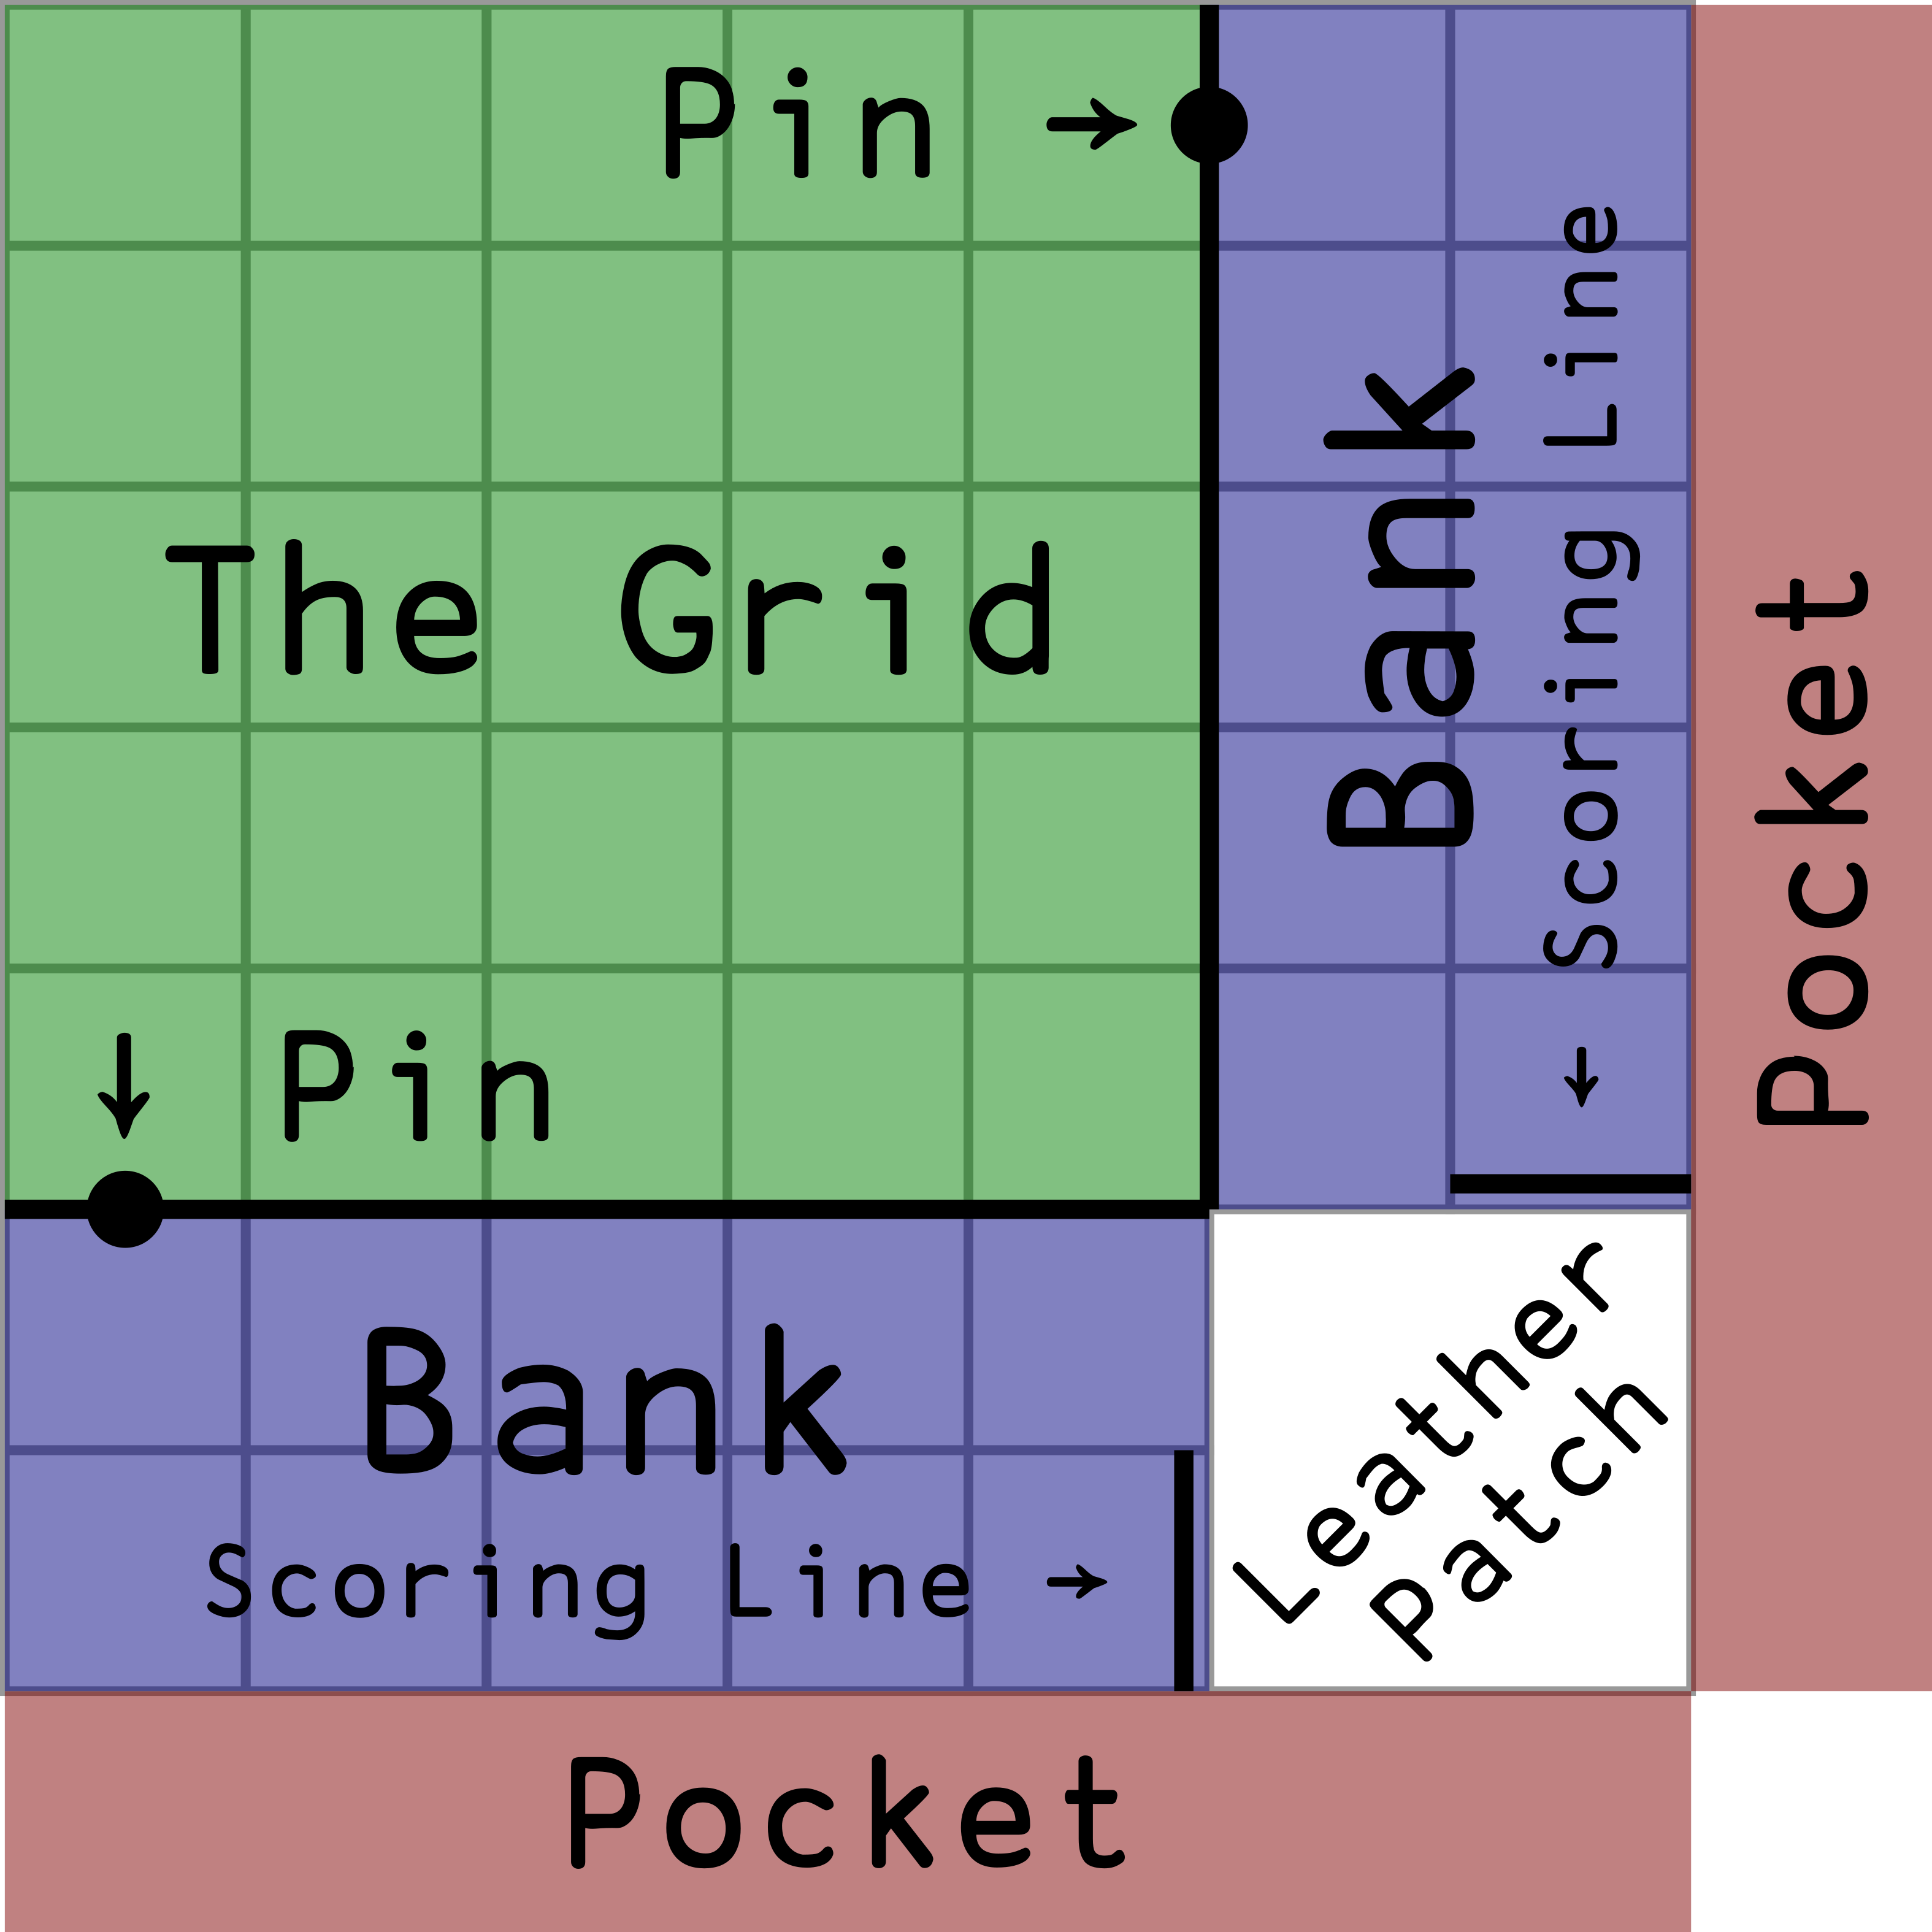
\includegraphics[width=8cm]{../graphics/zones}
    \caption{Board Anatomy}
    \label{fig:board-anatomy}
\end{figure}